\section{Entrepôts de données}\label{sec:rw:supervision:warehouse}
Pilier de l'informatique décisionnelle (\textit{Business Intelligence}), l'approche par entrepôt de données (\textit{Data Warehouses}) est très réputée et largement répandue. Son apport est originellement utilisé dans les applications pour entreprises. Toutefois, sa capacité de traitement et ses outils d'analyses ont permis son introduction dans d'autres cœurs de métiers tels que les réseaux~\cite{Gilbert:quicksand} ou l'agriculture~\cite{Abdullah:olap}. Cette architecture a été prévue pour permettre de fournir des outils d'analyses de données puissants. Pour cela, des procédés ont été développés pour permettre de faire de l'intégration de données hétérogènes, ainsi que des structures d'entrepôts prêts à répondre aux besoins d'analyses.

Son impact dans le cadre de la supervision semble clair. En effet, puisque l'observation et la compréhension du système passent par son analyse, des outils sont nécessaires pour effectuer ces opérations. L'établissement de diagnostic nécessite effectivement le parcours des données pour mieux comprendre les causes d'un problème. De plus, sa structure permettant l'intégration de donnée est à considérer pour intégrer les sources de données auxquelles nous sommes confrontés.

Par la suite, cette section détaille en premier lieu l'architecture globale de la solution. Nous détaillerons ensuite comment l'intégration est faite via les processus \textit{ETL}. Ensuite nous décrirons les structures de données utilisées pour permettre différentes analyses. Enfin, nous présenterons brièvement quelques outils d'analyses pouvant raisonner sur les données.

\subsection{Architecture globale}
La définition fonctionnelle d'un entrepôt de donnée est \enquote{\it une collection de données orientées sujet, intégrées, non volatiles et historisées, organisées pour le support d’un processus d’aide à la décision}~\cite{Inmon:warehouse}. Au sens large, un entrepôt est une base de données avec une organisation qui s'oriente avant tout sur l'application finale (l'analyse) plutôt que sur l'intégrité des données, et qui refuse la suppression ou la modification de données afin de garder une trace.
\begin{figure}[ht]
	\centering
	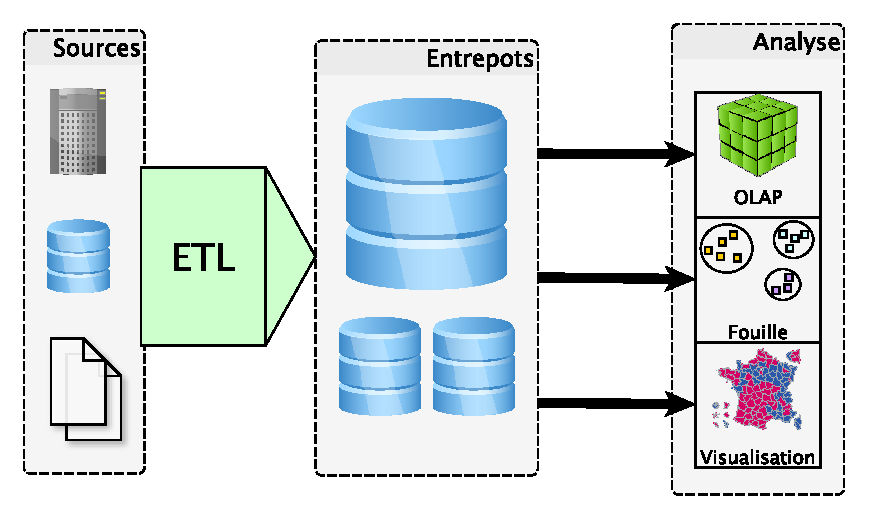
\includegraphics[width=0.75\textwidth]{rw-supervision-warehouses}
	\caption{Architecture globale d'une solution d'entrepôts de données}\label{fig:rw:supervision:warehouses}
\end{figure}
La figure~\ref{fig:rw:supervision:warehouses} présente une architecture abstraite des approches à entrepots. Les données sources sont supposées être dans des bases de données opérationnelles au mieux, ou à l'intérieur de fichiers bruts, au pire. À partir de ce constat, il est acté que les sources sont donc hétérogènes autant en terme de syntaxe que de sémantique.

Afin d'effectuer l'intégration des données à l'intérieur d'un (ou des) entrepôt(s), il faut traiter cette hétérogénéité et charger les données. Les processus \textit{ETL} ont été conçus pour cette tâche. Ces procédés sont découpés en trois phases : l'extraction (\textit{\textbf{E}xtract}), le traitement (\textit{\textbf{T}ransform}) et enfin le chargement (\textit{\textbf{L}oad}). Cet aspect sera détaillé en section~\ref{sec:rw:supervision:warehouse:etl}.

Par la suite, des outils d'analyses vont s'attacher aux entrepôts pour fournir les informations suffisantes à l'utilisateur pour qu'il puisse prendre une décision. Comme montré dans la définition des entrepôts, les bases de données sont orientées pour que ces outils d'analyses puissent effectuer leurs calculs nativement. La structure interne des entrepôts aura donc un impact sur la capacité des outils d'analyse.

\subsection{L'entrepôt et ses capacités}\label{sec:rw:supervision:warehouse:warehouse}
Les dépots de données ont pour but de stocker toutes les données relatives à un système. Son système de gestion est très souvent fait par un SGBD relationnel. C'est sa structure et ses opérations qui vont permettre une analyse pertinente.

Le cadre le plus récurrent pour les entrepôts de données est le traitement OLAP (\textit{Online Analytical Processing}). 
\subsubsection{OLAP et structure}
Le terme \textit{OLAP} a été d'abord défini en 1993 par le père du modèle relationnel, Edgar Codd, dans~\cite{Codd:olap}. Sa caractérisation est le fait de permettre le support \textit{d'analyse de données multidimensionnelles}. En effet, il apparait qu'une donnée représente un point dans un espace à plusieurs dimensions. L'exemple le plus commun dans ce domaine reste la gestion de vente pour une entreprise. La vente est un point dans l'espace $(Magasin, Produit, Temps)$ et sa valeur sera le prix (et/ou la quantité). 

D'un point de vue modélisation, le modèle en étoile ou en flocon permettent de structurer correctement un ensemble de données multidimensionnel dans le modèle relationnel~\cite{Levene:snowflake}. Le principe étant qu'il existe une relation des \textit{faits}. Celle-ci contiendra l'ensemble des données brutes. Dans notre cas, ce sera le prix. Cette relation est ensuite liée à plusieurs autres relations qui décrivent les différentes dimensions. Dans la structure en étoile, chaque dimension correspond à une relation. Dans le cadre de la structure en flocon, chaque dimension est un modèle relationnel normé (typiquement en forme normale de Boyce-Codd). 
\subsubsection{Le cube}
En 1995, les premiers concepts d'opérations multidimensionnelles arrivent avec le \textbf{cube}~\cite{Gray:cube}. Les dimensions doivent être définies de manière hiérarchique. Par exemple, un magasin (lieu) est située dans une ville, elle-même située dans un département, elle même située dans une région etc.. Par la suite, le traitement sur les données en elle-même va être centré sur la capacité à faire un agrégat. Dans notre cas, il est potentiellement intéressant de voir les résultats de vente par départements. Une somme est ainsi faite sur tous les résultats de chaque département.

L'hypercube \textit{OLAP} est la représentation des données multidimensionnelles. Dans notre cas, cela va être un vrai cube à trois dimensions : les magasins, les produits, et le temps comme représenté en figure~\ref{fig:rw:supervision:warehouses:cube}. Au début de l'analyse les dimensions sont discrétisées à leur plus haut niveau hiérarchique.
\begin{figure}[ht]
	\centering
	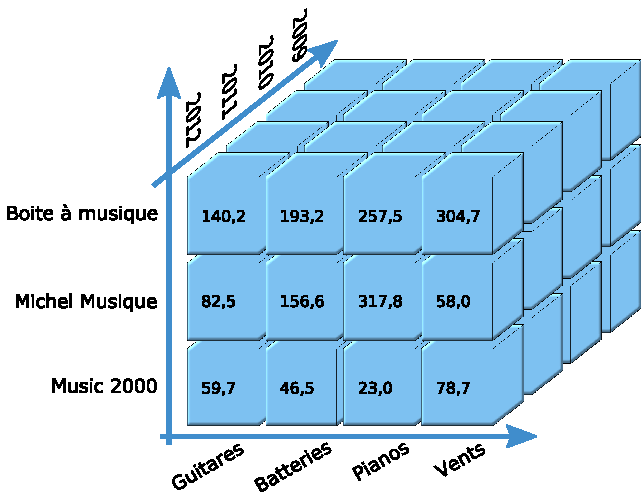
\includegraphics[width=0.75\textwidth]{rw-supervision-warehouses-cube}
	\caption{Représentation d'un cube \textit{OLAP} de trois dimensions, (\textit{Magasin}, \textit{Produit}, \textit{Temps}). Par exemple, en $2012$, le magasin \textit{Michel Musique} a vendu pour 156.6k\euro{} de batteries}\label{fig:rw:supervision:warehouses:cube}
\end{figure}
Cela forme un découpage du cube en autres cubies. Chacun de ces cubies contient la valeur d'un ou plusieurs agrégats choisis par l'utilisateur (ici, \textit{SUM}). Il est important de dire que l'utilisateur ne pourra pas que rarement exploiter correctement les $n$ dimensions de l'hypercube, car la représentation classique des données est sous forme de tableaux (donc 2 dimensions). Plusieurs opérations génériques existent sur ce cube pour que l'utilisateur puisse l'exploiter.

\subsubsection{Opérations}
\begin{itemize}
	\item[\textbf{Slice}] : Découpage du cube selon une des dimensions. Cela permet de retirer la complexité de l'analyse et de ne sélectionner qu'une partie des données selon un critère dimensionnel. Exemple : \textit{slice} du cube sur \textit{temps = 2012}.
	\item[\textbf{Dice}] : Extraction d'un sous-cube. Similaire à \textit{slice}, toutefois, la complexité n'est pas spécifiquement réduite car le nombre de dimension n'a pas changé. Exemple : extraction du cube pour les magasins \textit{La Boite à Musique} et \textit{Michel Musique}.
	\item[\textbf{Drill-down}] : Permet de faire la navigation à l'intérieur d'une dimension. Par exemple, le \textit{drill-down} du cube sur l'année \textit{2011} va couvrir la dimension du temps du 1er janvier 2011 jusqu'au 31 décembre 2011, en découpant la dimension par mois. Un autre \textit{drill-down} découpera en fonction des jours.
	\item[\textbf{Drill-up}] : Opération inverse de \textit{drill-down}. Ici, l'analyste remonte dans l'abstraction de la dimension de navigation (en passant d'une granularité par \textit{guitares} à \textit{instruments à cordes}).
	\item[\textbf{Pivot}] : Changement de perspective du cube. Jusqu'ici, le cube était représenté avec comme axes principaux $(Magasin, Produit)$. Le rapport à l'utilisateur se fait donc par ce biais principalement. Le pivot permet de tourner le cube pour changer ces axes.
\end{itemize}
L'opération \textit{roll-up} permet de calculer tous les agrégats à partir d'une ou plusieurs dimensions. Pour un tableau cela implique de calculer les agrégats par ligne, par colonne et au total. Ces outils sont extrèmement puissant en terme de pouvoir d'analyse.

D'un point de vue performance, les concepts de systèmes \textit{OLAP} optimisent les performances des manipulations sur le cube ainsi que les agrégats. Toutefois, si les requêtes sont trop complexes, les analyses peuvent prendre plusieurs minutes (ou pire, plusieurs heures).

\subsubsection{La visualisation : un domaine à part entière}
Permettre à l'utilisateur de pouvoir comprendre l'ensemble des données qui lui sont offerte est un domaine en soi~\cite{Maniatis:visualization}. En effet, être capable de rapporter correctement est technique car le nombre de dimensions manipulé peut être haut (bien au dessus de 10). Ce problème s'intensifie depuis l'avènement de la gestion des entrepôts spatio-temporels~\cite{Vaisman:spatiotemporal, Vaisman:continuous}. Dans ce type de systèmes, les données spatiales sont des polygones ou des lignes. La hiérarchie des dimensions est la partition des polygones. Les capacités d'analyses sont complexes car cela nécessite de faire des tests d'appartenances aux zones, ou pire, à des calculs d'intégrales sur les zones~\cite{Guting:movingobjects}.

Lors de la manipulation de concepts aussi visuels que la géographie, des outils doivent être capable de tracer les résultats d'analyses de manière claire visuellement et aussi d'interagir avec cette visualisation. Des outils ont étés proposés récemment pour pouvoir tracer une carte interactive capable de représenter l'exploration de données d'un cube spatio-temporel~\cite{Rivest:solap}.

Toutefois, l'exploration d'un cube de données ne fait pas partie des seules dispositions d'un entrepôt de données.
\subsubsection{La fouille}
La fouille de données (\textit{Data Mining}) est le procédé permettant d'extraire de nouvelles connaissances à partir d'un grand ensemble de données. Les principes sont essentiellement dirigés par l'utilisation de nombreuses méthodes et algorithmes spécialisés. Deux grandes catégories se dessinent toutefois :
\begin{itemize}
    \item[\textit{Descriptif}] : Aussi connu en tant qu'analyse de données statistiques. Le but étant d'être capable de classer, et de simplifier des données multidimensionnelles afin d'aider la compréhension de l'information.
    \item[\textit{Prédictif}] : Le but étant d'être capable d'expliquer ou de prévoir un phénomène qui a été mesuré.
\end{itemize}
Il est important de remarquer que ces approches sont d'excellents compléments à l'observation. L'entrepôt de données est en mesure de fournir suffisamment de données pour permettre ce genre d'analyse par la suite.

Nous avons vu que les entrepôts permettent de stocker et d'analyser un grand ensemble de données. Toutefois, ces données doivent être chargées à l'intérieur de ce dépôt.
\subsection{L'intégration par ETL}\label{sec:rw:supervision:warehouse:etl}
Afin de charger les données provenants de sources hétérogènes dans un entrepôt, l'architecture la plus utilisée reste l'utilisation de processus \textit{ETL} (\textit{Extract}, \textit{Transform}, \textit{Load}). L'ensemble forme un ensemble de tâche à exécuter périodiquement où sur impulsion. Le développement de ces processus est une partie importante de la mise en œuvre d'un système à base d'entrepôt, généralement coûteuse en terme de mise en œuvre, à cause de sa complexité.
\subsubsection{Extraction}
Les données sont d'abord extraites des sources hétérogènes. L'extraction peut se faire sous différentes formes suivant les sources, ainsi il est souvent nécessaire d'aligner le format source à un format commun. L'utilisation de base de données intermédiaires (\textit{staging}) est une solution pour les importations complexes.

\subsubsection{Transformation}
Cette partie est sûrement la plus complexe de toutes. L'idée étant évidemment d'aligner les données d'entrée dans le schéma et la sémantique de (ou des) entrepôts. Les opérations courantes pouvant remplir différentes fonctions : nettoyage, applications de règles, vérification d'intégrité, jointure, agrégats, conversion de type. 

Le principe global reste d'être axé sur la composition d'opérateurs comme montré dans la figure~\ref{fig:rw:supervision:warehouses:etl}. Toutefois, il n'existe pas de standard ou d'algèbre permettant de décrire ces différents opérateurs~\cite{Vassiliadis:taxonomy}. En effet, les opérateurs du modèle relationnel permettent de faire certaines des opérations. Seulement des opérations telles que l'alignement de valeurs (\textit{Homme} vers \textit{Masculin} par exemple), la génération de clé, la séparation de colonnes ou autre transformation de données complexes ne sont pas gérées par les primitives de ce modèle. Il faut rajouter des extensions. 

\begin{figure}[ht]
    \centering
    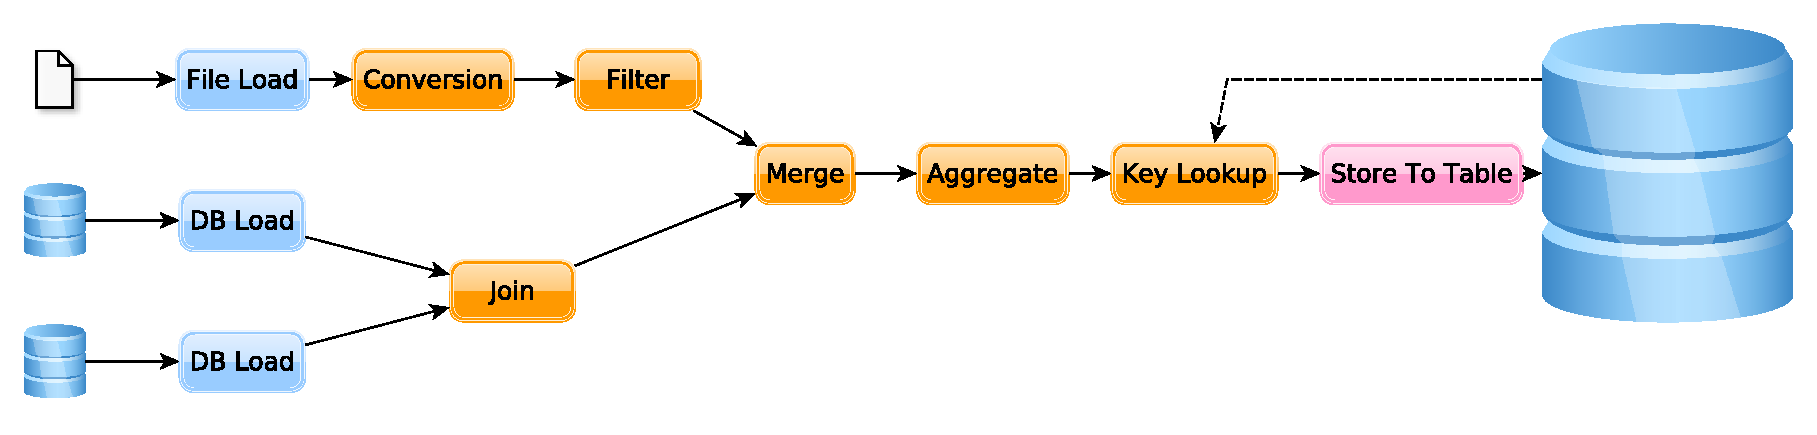
\includegraphics[width=0.9\textwidth]{rw-supervision-warehouses-etl}
    \caption{Exemple de processus ETL}\label{fig:rw:supervision:warehouses:etl}
\end{figure}


Ces opérateurs sont de cardinalité $1\!\!:\!\!1$, $n\!\!:\!\!1$, $1\!\!:\!\!n$ ou $n\!\!:\!\!n$, mais leur fonctionnalité est très dépendante des différents constructeurs de système ETL. Plusieurs travaux récents s'intéressent à dresser une taxonomie~\cite{Vassiliadis:taxonomy} de ces différents opérateurs. Des approches~\cite{Akkaoui:etl,Trujilo:uml-etl} s'intéressent ensuite à fournir des outils permettant de pouvoir développer des processus \textit{ETL} de façon indépendante au système. Ceci étant possible grâce aux techniques de transformations de modèles.

\subsubsection{Chargement}
Le chargement permet la publication des nouvelles données fraîchement traitées à l'intérieur de l'entrepôt. Plusieurs considérations de performances rentrent en compte pour savoir quand la publication sera effective. En effet, lors d'une mise à jour de base de donnée relationnelle, le système transactionnel requiert que les données soient à jour à la fin de la transaction. Ici, l'écriture effective peut-être retardée pour permettre un chargement des données moins coûteux~\cite{Petit:historical}.

De plus, à cet étape, il est courant de générer des rapports compilant les données transformées vers un document qui sera transmit à l'utilisateur.

\subsubsection{Le temps réel : un nouveau challenge}
La fraicheur des données à l'intérieur d'un entrepôt de donnée n'a pas été une contrainte critique jusqu'ici. Les latences usuellement visées par ce type d'approche sont au alentour de l'heure voire de jours~\cite{Oracle:realtimedw}. Récemment, des travaux se sont intéressés à améliorer la qualité du traitement en terme de fraicheur de données (pour passer à l'ordre de la minute voire de la seconde).

Comme présenté en section~\ref{sec:intro:problematique}, la gestion de l'évolution des données est important dans notre cadre. Ici, le dynamisme n'est pas explicite car il n'y a pas de mécanisme d'événement. Ainsi, il est nécessaire d'implémenter un \textit{CDC} (\textit{Change Data Capture}) capable de transmettre les nouvelles données via un canal de communication dédié.

Plusieurs systèmes commencent à supporter la gestion en temps réel de l'import de données~\cite{Thomsen:rite, Oracle:ODI}. Toutefois, il n'y a pas de résultats concrêts concernant le traitement des données dynamiques en tant que tel. Par exemple, la définition d'agrégat sur une fenêtre de temps doit se faire à la main via une base de données intermédiaire.

\subsection{Synthèse}
\begin{table}[!ht]
\criteretabDonnee
    {Modèle relationnel}
    {Géré par le modèle relationnel. Modélisation en étoile et par normalisation.}
    {Faible gestion du dynamisme en dehors des mécanismes CDC dans les entrepôts temps-réels.}
\criteretabTraitement
    {Instantané principalement. Les ETL peuvent être apparentés à des interrogations continues.}
    {Intégration complexe via les ETL.}
    {Paradigme déclaratif pour l'exploration de données. Algorithmique pour la fouille de données. Principalement procédural pour les ETL.}
    {En dehors des algorithmes et des procédures de gestion de syntaxe ou de règles métiers, le traitement des données est dérivé de l'algèbre relationnel.}
\criteretabAdaptabilite
    {Spécification du schéma de l'entrepôt. Description des processus ETL. Si les besoins d'analyses sont poussés, il est nécessaire de concevoir les outils d'analyse aussi.}
    {La gestion de données multidimensionnelles apporte cette gestion de perspective de façon native. Il est possible de créer différents sous-entrepôts pour chacun des métiers avec des données agrégées (alimentés par ETL).}
    {Il est très souvent nécessaire de rajouter des opérateurs, ou des logiciels d'analyses plus poussés. Les implémentations permettent en général de rajouter des procédures personnalisés à tout les niveaux de la chaîne.}
    {Les procédés sont lourds et complexes et la durée de réactivité peut se compter en minutes ou en heures. Toutefois, ces systèmes manipulent des Tera de données.}
\caption{Synthèse des entrepôts de données}\label{tab:rw:supervision:warehouses:synthese}
\end{table}
En conclusion, les entrepôts de données représentent une grande capacité de traitement des données. Sa prise en charge de données historique et ses pouvoirs d'analyses sont précieux pour l'observation de système. Toutefois, le processus d'intégration est trop lent pour pouvoir gérer des alertes. De plus, il existe une ambiguïté sémantique sur les opérateurs disponibles qui dépendent du système.
